
% ============================================================================================================

% JOURNAL MODE
% ------------

\documentclass[extra]{gji}
\setlength{\paperwidth}{210mm}
\setlength{\paperheight}{297mm}% fixed.
\usepackage[pass]{geometry}\usepackage{timet}

% ============================================================================================================

% MANUSCRIPT MODE
% ---------------

% \documentclass[extra,mreferee]{gji}

% ============================================================================================================

% \addtolength{\paperheight}{1in}

\usepackage{fancyhdr}
\usepackage{comment}
\usepackage{color}
\usepackage{graphicx}
\usepackage{amsmath}
\usepackage{mathtools}
\usepackage{environ}
\usepackage{datatool}
\usepackage{textcomp}


% \widowpenalty=1000
% \clubpenalty=1000


\title[% 
Validation with attenuation Relationship
% 
]{% 
Toward a Framework for Ground Motion Simulation Validation using Attenuation Relationships. Part1: Calibration Between NGA-West2 Predictions, Physics-Based Synthetics, and Data
% 

}
\author[R.~Taborda {\rm et al.}]{% 
Ricardo Taborda,$^{1,2}$\thanks{Corresponding author: ricardo.taborda@memphis.edu}
Shima Azizzadeh-Roodpish,$^{1,2}$\vspace{0.5ex} \\ \normalfont{\LARGE and Naeem Khoshnevis,$^{2}$} \vspace{1ex} \\
% 
$^1$ Department of Civil Engineering, University of Memphis, Memphis, TN \emph{38152}, USA\\
$^2$ Center for Earthquake Research and Information, University of Memphis, Memphis, TN \emph{38152}, USA
% 
}
% \date{Received 2015 August 1; in original form 2015 July 1}
\date{To be submitted by March, 2016}
\pagerange{\pageref{firstpage}--\pageref{lastpage}}
\volume{000}
\pubyear{0000}

%\def\LaTeX{L\kern-.36em\raise.3ex\hbox{{\small A}}\kern-.15em
%    T\kern-.1667em\lower.7ex\hbox{E}\kern-.125emX}
%\def\LATeX{L\kern-.36em\raise.3ex\hbox{{\Large A}}\kern-.15em
%    T\kern-.1667em\lower.7ex\hbox{E}\kern-.125emX}
% Authors with AMS fonts and mssymb.tex can comment out the following
% line to get the correct symbol for Geophysical Journal International.

\let\leqslant=\leq

\newtheorem{theorem}{Theorem}[section]


\newcommand{\vsmin}{$V_{S_{\min}}$}
\newcommand{\vsmineq}[1]{$V_{S_{\min}}=#1$~m/s}
\newcommand{\vsthirty}{$V_{S30}$}
\newcommand{\vs}{$V_{S}$}
\newcommand{\vseq}[1]{$V_{S}=#1$~m/s}

\newcommand{\vp}{$V_{P}$}
\newcommand{\vpeq}[1]{$V_{P}=#1$~m/s}

\newcommand{\qp}{$Q_{P}$}
\newcommand{\qs}{$Q_{S}$}

\newcommand{\fleq}[1]{$f\leq#1$~Hz}
\newcommand{\fmax}{$f_{_{\max}}$}
\newcommand{\fmaxeq}[1]{$f_{_{\max}}=#1$~Hz}

\newcommand{\eqmag}[1]{$M_{#1}$}

\newcommand{\adomain}[3]{#1~#3 $\times$ #2~#3}
\newcommand{\vdomain}[4]{#1~#4 $\times$ #2~#4 $\times$ #3~#4}


\begin{document}

\label{firstpage}

\maketitle


\section{Introduction}

Increasing advances in ground motion simulation emboldens researches to seek for reliable methods of simulation validation. Validation is an effort to check the correctness of the formulation and the accuracy with respect to observations. The concept of simulation has found its way from systems science  (e.g. Sargent, 2005; Oberkampf et al., 2004) to earthquake simulation community (e.g., Bielak et al.,2010; Chaljub et al., 2010). Up untill now, validaton of ground motion simulations is done by comparing synthetic seismograms against observations from past earthquakes (Olsen and Mayhew, 2010; Taborda and Bielak, 2013 and 2014, Taborda et al., 2016) predominantly using quantitative methods known as goodness-of-fit (GOF) or misfit criteria (\citet{Anderson_2004_Proc}; Olsen and Mayhew, 2010; Kristekova et al., 2009). These validations are concentrating comparisions to the availability of data, which for most of the past events is limited to a reduced number of locations.\par
However, the simulations are resulved for the whole computational domain, not just the specific stations, and this provide us with a complete surface datsets which can be used to build simulation specific attenuation curves comparable to well-established attenuation relationships.The goal of this project is to shape a new simulation validition framework based on comparision with attenuation relationships. To this end, we start with the available recorded data for southern california region from past earthquakes and synthetics from four different velocity model to define and calibrate a goodness of fit criteria using their corrisponding attenuation relationships. Later we will extend the findings to the whole simulation domain and will perform the evaluation between NGA-West2 prediction and our physic-based synthetics.  



\section{Data and Synthetic}

Considered Data for conducting this study contains thirty moderate-magnitude earthquakes ($3.5 > M_w > 5.5$) occurred between 1998 and 2014. The latest version of ground motion prediction equations (GMPEs) database includes small-to-moderate earthquakes in California which will be helpful in calibration of compariosion criteria. 
Selected events are spread throughout a simulation domain with a volume projection of \vdomain{180}{135}{62}{km}, which covers the entire Los Angeles metropolitan area and most of the significant geologic structures around. Fig.~\ref{fig:region} shows the simlation domain in which we labled the events with sequential letter code from A to Z and AA to AD and Table \ref{tab:events} provides detailed information for those selected events.The unprocessed recorded data from Southern California Earthquake Data Center (SCEDC) and Center for Engineering Strong Motion Data (CESMD) are downloaded for each of the earthquakes to take advantage of the numerous time series available from different data centers. We obtained records for moree than 800 stations, Some of which were in common between different networks and some were not usable. Records from SDEDC and CESMD were processed and selected for each event. we performed gain and baseline corrections, and applied a high-pass filter at 0.05 Hz before integrating to obtain velocities and displacements. The final number of chosen records for validation for any of the selected earthquake can be found in Table \ref{tab:events}.

\begin{figure*}
    \centering
    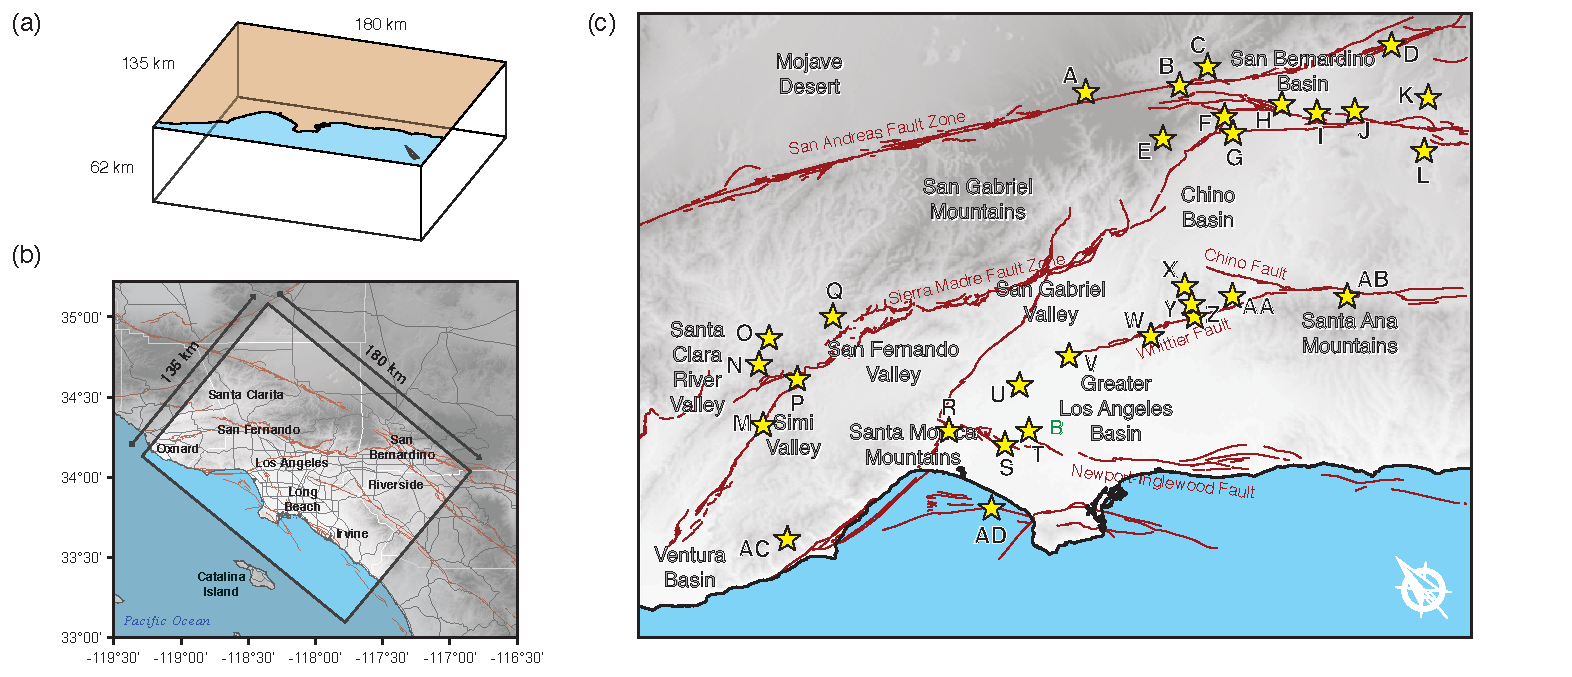
\includegraphics
    	[width=\textwidth]
    	{figures/pdf/figure-01}
    \caption{Region of interest and simulation domain. (a) 3D view of the simulation domain. (b) Geographical location and surface projection of the simulation domain, along with the names of the main cities surrounding the Los Angeles metropolitan are. (c) Major geologic structures including basins, valleys and mountains, along with the main quaternary faults in the region. The color background represents the surface \vsthirty{} values included in the CVM-H+GTL model, with a topography shading effect.}
    \label{fig:region}
\end{figure*}


\begin{table*}
	\centering\small
	\caption{Selected events with their ID \citet{SCEC} and description of source location, magnitude, focal mechanism (strike, dip, and rake angles) \citet{Lee_2011_GJI}, and date and time (in coordinated universal time, or UTC).}
	\begin{tabular}[t]{@{} c l r c r@{, }l r c c c r}
	\\[-3ex]
	\hline
	  	Code								& 
	  	Earthquake name						&
	  	Event ID							& 
	  	\eqmag{w}							&
	  	\multicolumn{2}{c}{Coordinates}		&
	  	Depth								&
	  	Strike/Dip/Rake						&
	  	Date								&
	  	UTC Time							&
	  	Num.								\\
	  										& 
	  										&	
	  										& 
	  										&	
	  	\multicolumn{2}{c}{(lon., lat.)} 	&
	  	(km)								&	
	  										&
	  	(yyyy/mm/dd)						&
	  	(hh:mm:ss)							&
	  	Stns.\\
	\hline																																
		A	& Wrightwood			&	 9064568	&	4.40	&	--117.6480	&	34.3740	&	 8.99	&	285/57/86	&	1998/08/20	&	23:49:58.198	&	17	\\ % A 
		B	& NW of Devore			&	10972299	&	3.79	&	--117.4642	&	34.2655	&	10.91	&	 98/58/68	&	2001/07/19	&	20:42:36.470	&	52	\\ % R
		C	& NNE of Devore			&	14494128	&	3.72	&	--117.3838	&	34.2587	&	 7.18	&	344/69/-33	&	2009/08/01	&	12:55:55.317	&	77	\\ % Z
		D	& Yucaipa				&	14155260	&	4.88	&	--117.0113	&	34.0580	&	11.61	&	 75/59/55	&	2005/06/16	&	20:53:26.225	&	172	\\ % V
																					
		E	& N of Rancho Cucamonga	&	10216101	&	3.60	&	--117.5762	&	34.2058	&	 4.92	&	 54/69/16	&	2006/11/04	&	19:43:44.376	&	55	\\ % J
																					
		F	& 2002 Fontana			&	13692644	&	3.74	&	--117.4288	&	34.1613	&	 6.54	&	233/72/-28	&	2002/07/25	&	00:43:14.872	&	55	\\ % S
		G	& 2005 Fontana			&	14116972	&	4.42	&	--117.4387	&	34.1250	&	 4.15	&	222/88/-25	&	2005/01/06	&	14:35:27.593	&	83	\\ % U
		H	& San Bernardino		&	10370141	&	4.45	&	--117.3042	&	34.1073	&	14.22	&	 87/70/28	&	2009/01/09	&	03:49:46.051	&	159	\\ % L
		I	& N of Loma Linda		&	 9140050	&	4.37	&	--117.2525	&	34.0500	&	15.36	&	270/90/-6	&	2000/02/21	&	13:49:43.017	&	38	\\ % D
		J	& Redlands				&	10541957	&	4.10	&	--117.1797	&	34.0045	&	 8.53	&	 33/46/-68	&	2010/02/13	&	21:39:06.349	&	97	\\ % Q
		K	& 2010 Beaumont			&	10530013	&	4.28	&	--117.0232	&	33.9322	&	13.93	&	234/89/9	&	2010/01/16	&	12:03:25.345	&	76	\\ % P
		L	& 2006 Beaumont			&	14239184	&	3.90	&	--117.1122	&	33.8560	&	11.53	&	 45/31/-25	&	2006/07/10	&	02:54:43.809	&	66	\\ % W
																					
		M	& Simi Valley			&	14000376	&	3.59	&	--118.7530	&	34.2722	&	13.81	&	234/62/60	&	2003/10/29	&	23:44:48.206	&	54	\\ % T
		N	& WSW of Valencia		&	 9753489	&	3.90	&	--118.6678	&	34.3705	&	14.21	&	 83/62/57	&	2002/01/29	&	06:00:39.140	&	52	\\ % H
		O	& N of Pico Canyon		&	 9096972	&	3.98	&	--118.6090	&	34.3980	&	11.53	&	287/55/54	&	1999/07/22	&	09:57:23.502	&	26	\\ % C
		P	& Chatsworth			&	14312160	&	4.66	&	--118.6195	&	34.2995	&	 7.58	&	 82/27/51	&	2007/08/09	&	07:58:48.888	&	109	\\ % X
		Q	& Newhall				&	15237281	&	3.86	&	--118.4580	&	34.3508	&	 3.59	&	236/58/33	&	2012/10/28	&	15:24:23.172	&	120	\\ % AC
																					
		R	& Beverly Hills			&	 9703873	&	4.24	&	--118.3885	&	34.0590	&	 7.90	&	262/81/4	&	2001/09/09	&	23:59:17.695	&	130	\\ % F
		S	& Inglewood Area		&	10410337	&	4.70	&	--118.3357	&	33.9377	&	13.86	&	243/60/25	&	2009/05/18	&	03:39:36.126	&	213	\\ % O
		T	& NW of Compton			&	 9716853	&	3.98	&	--118.2702	&	33.9290	&	21.13	&	116/68/71	&	2001/10/28	&	16:27:45.388	&	55	\\ % G
																					
		U	& Downtown Los Angeles	&	 9093975	&	3.77	&	--118.2180	&	34.0100	&	 9.53	&	125/49/79	&	1999/06/29	&	12:55:00.371	&	25	\\ % B
																					
		V	& Whittier Narrows		&	14601172	&	4.44	&	--118.0817	&	33.9923	&	18.85	&	282/36/73	&	2010/03/16	&	11:04:00.026	&	180	\\ % AA
		W	& La Habra				&	15481673	&	5.10	&	--117.9300	&	33.9220	&	 5.00	&	239/70/38	&	2014/03/29	&	04:09:42.970	&	311	\\ % AD
		X	& Chino Hills			&	14383980	&	5.39	&	--117.7613	&	33.9530	&	14.70	&	 47/51/32	&	2008/07/29	&	18:42:15.960	&	335	\\ % Y
		Y	& 2002 Yorba Linda		&	 9818433	&	4.75	&	--117.7758	&	33.9173	&	12.92	&	 34/84/-10	&	2002/09/03	&	07:08:51.675	&	67	\\ % I
		Z	& 2009 Yorba Linda		&	10399889	&	3.98	&	--117.7892	&	33.8940	&	 4.23	&	208/65/26	&	2009/04/24	&	03:27:49.840	&	91	\\ % M
		AA	& ESE of Yorba Linda	&	 9644101	&	3.64	&	--117.6882	&	33.8777	&	 3.59	&	 56/65/37	&	2001/04/13	&	11:50:11.916	&	53	\\ % E
																					
		AB	& Lake Elsinore			&	10275733	&	4.73	&	--117.4770	&	33.7322	&	12.60	&	 65/59/58	&	2007/09/02	&	17:29:14.827	&	116	\\ % K
																					
		AC	& Westlake Village		&	10403777	&	4.42	&	--118.8825	&	34.0667	&	14.17	&	254/73/30	&	2009/05/02	&	01:11:13.084	&	94	\\ % N
																					
		AD	& Hermosa Beach			&	14738436	&	3.69	&	--118.4578	&	33.8572	&	11.23	&	 57/41/54	&	2010/06/07	&	23:59:27.165	&	93	\\ % AB
	\hline
	\end{tabular}
	\label{tab:events}
\end{table*}




The simulations of the selected events are all done for the four major velocity models currently available for the region of southern California: CVM-S4, CVM-S4.26, CVM-H and CVM-H+GTL. 3D simulations with point source model are done at maximum frequency of 1 Hz and minumum shear wave velocity of 200 m/s for each earthquake and velocity model combination using Hercules, a parallel 3D finite element computer application for solving forward anelastic wave propagation problems which has been thoroughly tested and verified in multiple supercomputers. All the runs are done on Blue Waters at the National Center for Supercomputing Applications.

Using a developed python code, we collect the results of the Peak Ground Acceleration (PGA), Peak Ground Velocity (PGV), and Peak Ground Displacement (PGD) in three directions (EW, NS, Up), for all the events in all available stations for both synthetics and data. This information will be used later in validation method.



\section{Evaluation Method}

Attenuation relationship relates the distance from source to the ground motion features such as PGA, PGV and PGD.  Plotting this data for different stations in the logarithmic scale for different cases suggest that attenuation relationship can initially be approximated by a single line. So we will use linear regression ( straight line-first order polynomial degree regression model) for both data and synthetics. $b$ is the slope of the regression line, ($y=a+bx+\epsilon$, being $\epsilon$ the error rodisturbance term associated to that model and $a$ the intercept), which can be calculated by equation (\ref{eq:a}). Later, if necessary, we can expand this concept to a bilinear approximation for a better fit. 


%
\begin{equation}
	\mathrm{b} = \left( 
		\frac{\sum\limits_{i=1}^n ((x_i-\bar{x})(y_i-\bar{y}))}{\sum\limits_{i=1}^n (x_i-\bar{x})^2} 
	\right)
	\hspace{0.25em}.
	\label{eq:a}
\end{equation}

For camparing two lines, there are two components to be considered. The distance of two lines (we call it "Amplitude score") and their slope (we call it "Rate score").The evaluation process proposed here is based on defining a goodness-of-fit criteria for these two aspects. 

For comparing the difference between the amount of peak ground characteristic of data and synthetics at each station, the goodness-of-fit (GOF) criteria (peak acceleration (C5), peak velocity (C6), peak displacement (C7)) proposed by \citet{Anderson_2004_Proc} is used. For these GOF scale, Each parameter is mapped onto a numerical scale ranging from 0 to 10, with 0 for the worsth and 10 for the best match between two signals.
Any of the C5, C6 and C7 score can be calculated by equation (\ref{eq:s}).

%
\begin{equation}
	\mathrm{S(p_1,p_2)} = 10exp \left( 
		-(\frac{p_1 - p_2}{min(p_1,p_2)})^2
	\right)
	\hspace{0.25em}.
	\label{eq:s}
\end{equation}

There are many benefits in using this function for calculating score. The function is monotonically decreasing as the difference between the parameters increase. It is symmetrical and because of that the score is similar regrdless of the order of bigger or smaller values. Multiplying the factor of 10 puts the score into a comfortable range of value for giving a score between 0 and 10. Small differences are not penalized too severely since it is an exponential function. We calculate this GOf at each station and find their average and assign that amount as the "amplitude score". 

To define a GOF score for the differences in the slope of two lines, There are some statistical approach available. We suggest to use the Student's t-test based on the standard error of regression models according to an article by Andre and Estevez-Perez (2014). The advantages of using t-test is that this parameter not only considers the different slopes, but also is affected by the number of available data and synthetics and the standard deviation of the ground motion parameters. Generally, when there is a goofd fit of slope, the t has lower amount. Lower number of stations and higher stdv will increse the value of t. This will serve as a good factor for defining a GOF function for slope comparision. For that, certain amount of judgment will be needed to define the tren and to choose the necessary levels which should not be considered useful fits for engineering applications.

Most t-test statistics can be formulated as $t_{experimetal}= \frac{(\hat{\theta}-\theta)}{SE}$, being $\theta$ a population parameter, $\hat{\theta}$ an estimator of ${\theta}$ and $SE$ the standard error of the estimator ( or equivalently, an estimation of the standard deviation of the estimator). The test statistic is equation (\ref{eq:t}).

%
\begin{equation}
	\mathrm{t} = \left( 
		\frac{b_1 - b_2}{s_{b_1-b_2}}
	\right)
	\hspace{0.25em}.
	\label{eq:t}
\end{equation}

where

%
\begin{equation}
	\mathrm{s_{b_1-b_2}} = \left( 
		s_{Res}\sqrt{\frac{1}{s_{x_1}^2(n_1-1)}+\frac{1}{s_{x_2}^2(n_2-1)}}
	\right)
	\hspace{0.25em}.
	\label{eq:sbb}
\end{equation}

being $n_1$ and $n_2$ the sample sizes for each sample datta and $s_{x_1}$ and $s_{x_2}$ standard deviations. $s_{Res}$ is a unique estimator which is a weighted average of two variances (alos known as $s_{pool}$ since by that we can pool the estimates of the error variances, weightening each by their degrees of freedom) and can be calculated from equation (\ref{eq:res}).

%
\begin{equation}
	\mathrm{s_{Res}^2} = \left( 
		\frac{(n_1-2)s_{y,x_1}^2+(n_2-2)s_{y,x_2}^2}{(n_1-2)+(n_2-2)}
	\right)
	\hspace{0.25em}.
	\label{eq:res}
\end{equation}


in that, $s_{y,x_1}$ and $s_{y,x_2}$ are the residual variance (often known as squared standard error of the regression), which estimates the variance of the regression or variance of the model from the experimental data. Using above euation we can find the rate score of each pair of regression lines.

There can be different approaches in the way of combination of amplitude and rate score. We can use simple average or also give weight to each score and calculate a weighted average. In this report, we simply considered the total average as simple average of two calculated scores.  





\section{Results}

Here, We have the result of quantitative measures to assess the level of agreement between the data and the simulation, using amplitude and slope parameters. A python program is developed to produce plots of all the available pairs of data and synthetics attenuation relationship comparision, and also to compare all four velocity models together.Fig.~\ref{fig:pgv} shows results of PGV in total (average of 3 directions) for all 4 models as an example. As it can be seen, the four models have close regression lines in most of the cases.

\begin{figure*}
    \centering
    \includegraphics
    	[width=\textwidth]
    	{figures/pdf/figure-02}
    \caption{PGV for all the 30 events and all four models are presented.}
    \label{fig:pgv}
\end{figure*}

For the first set of trials the t prameter was calculated. Then, considering the variations in the t value ranges, an initial score is proposed corresponding to each t. Current selected ranges are equal to  $1/t \leq 10$ It will be an acceptable function of t for calculating score instead of just assigning the score for different t ranges. This will make the GOF more accurate and applicable.

In order to better see the changes in amplitude score, rate score, and total score using a python program plots for the trend of changes in all 30 events are produced. Here some of them are discussed with the aim of comparing four different velocity models. Fig.~\ref{fig:amp} shows trend of amplitude score for PGD, PGV and PGA for all 4 models. In all of them the same trend is visible. PGD has better scores, then PGV, then PGA. Among all cvms426-223 has better overall result.

\begin{figure*}
    \centering
    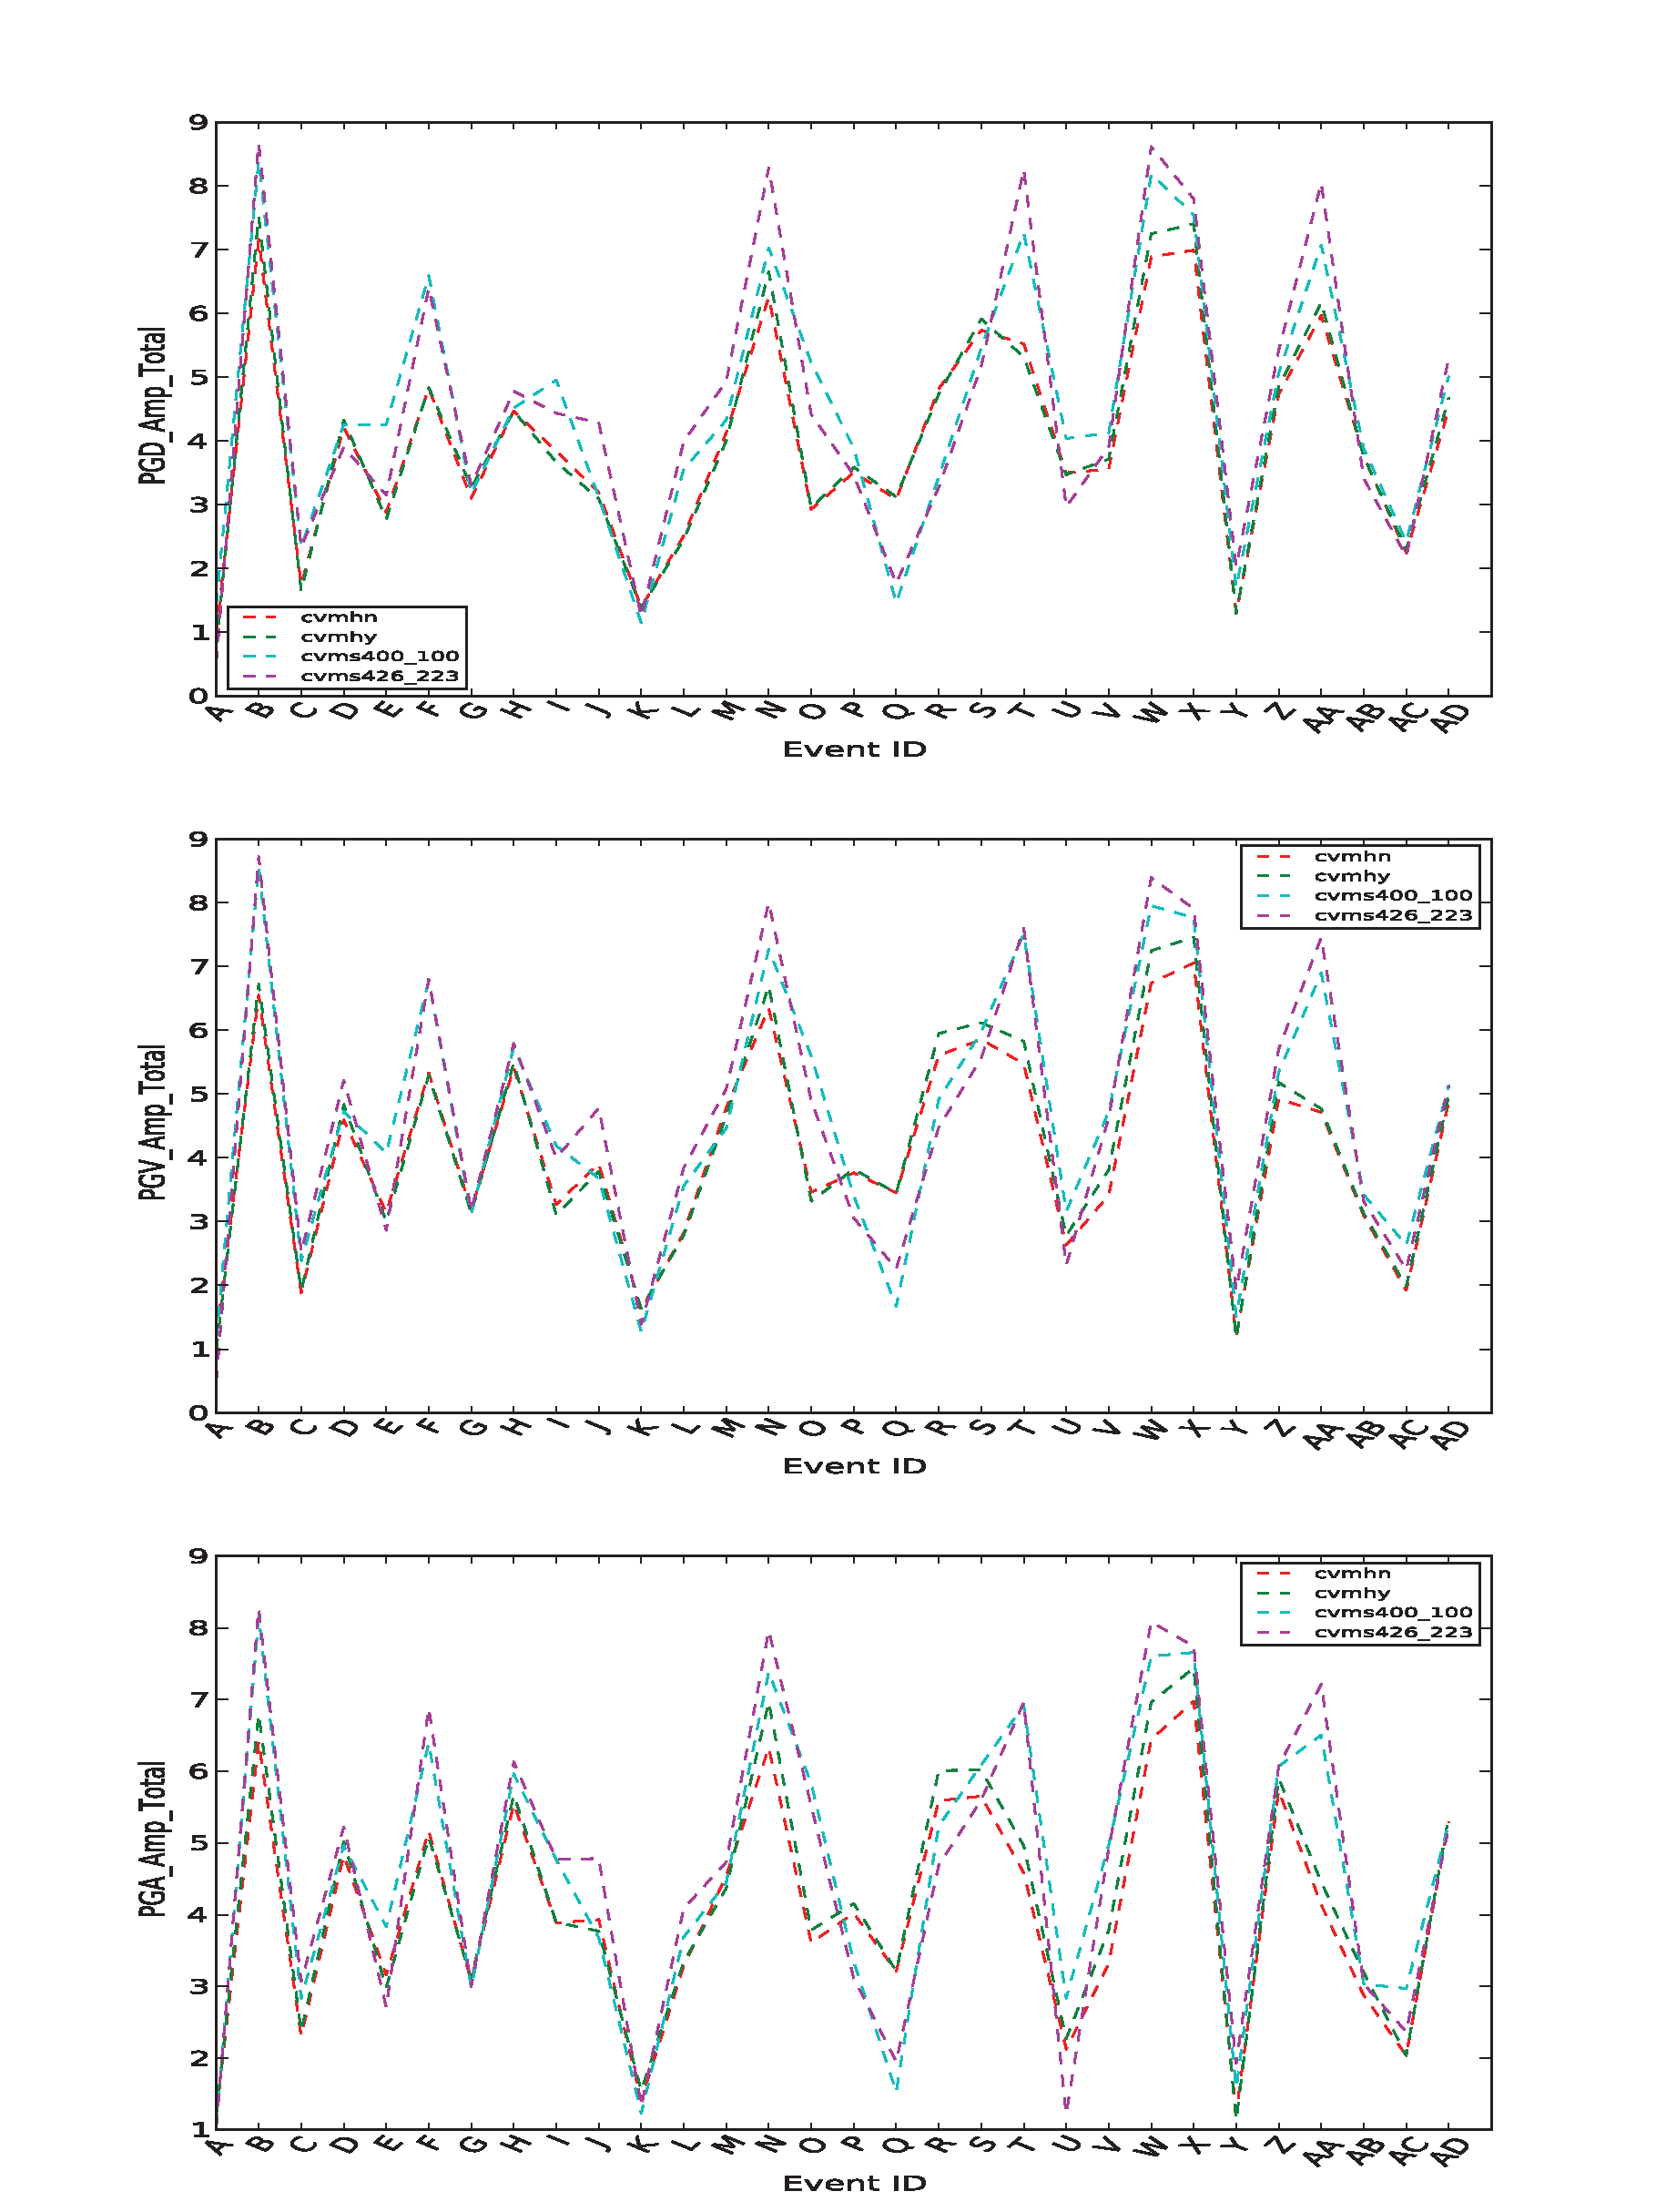
\includegraphics
    	[width=\textwidth]
    	{figures/pdf/figure-03}
    \caption{PGD, PGV and PGA amplitude score for all the 30 events and all four models are presented.}
    \label{fig:amp}
\end{figure*}

 Fig.~\ref{fig:rate} shows trend of rate score for PGD, PGV and PGA for all 4 models. PGD still has better scores then PGV, then PGA. Bur we can see different trends here.

\begin{figure*}
    \centering
    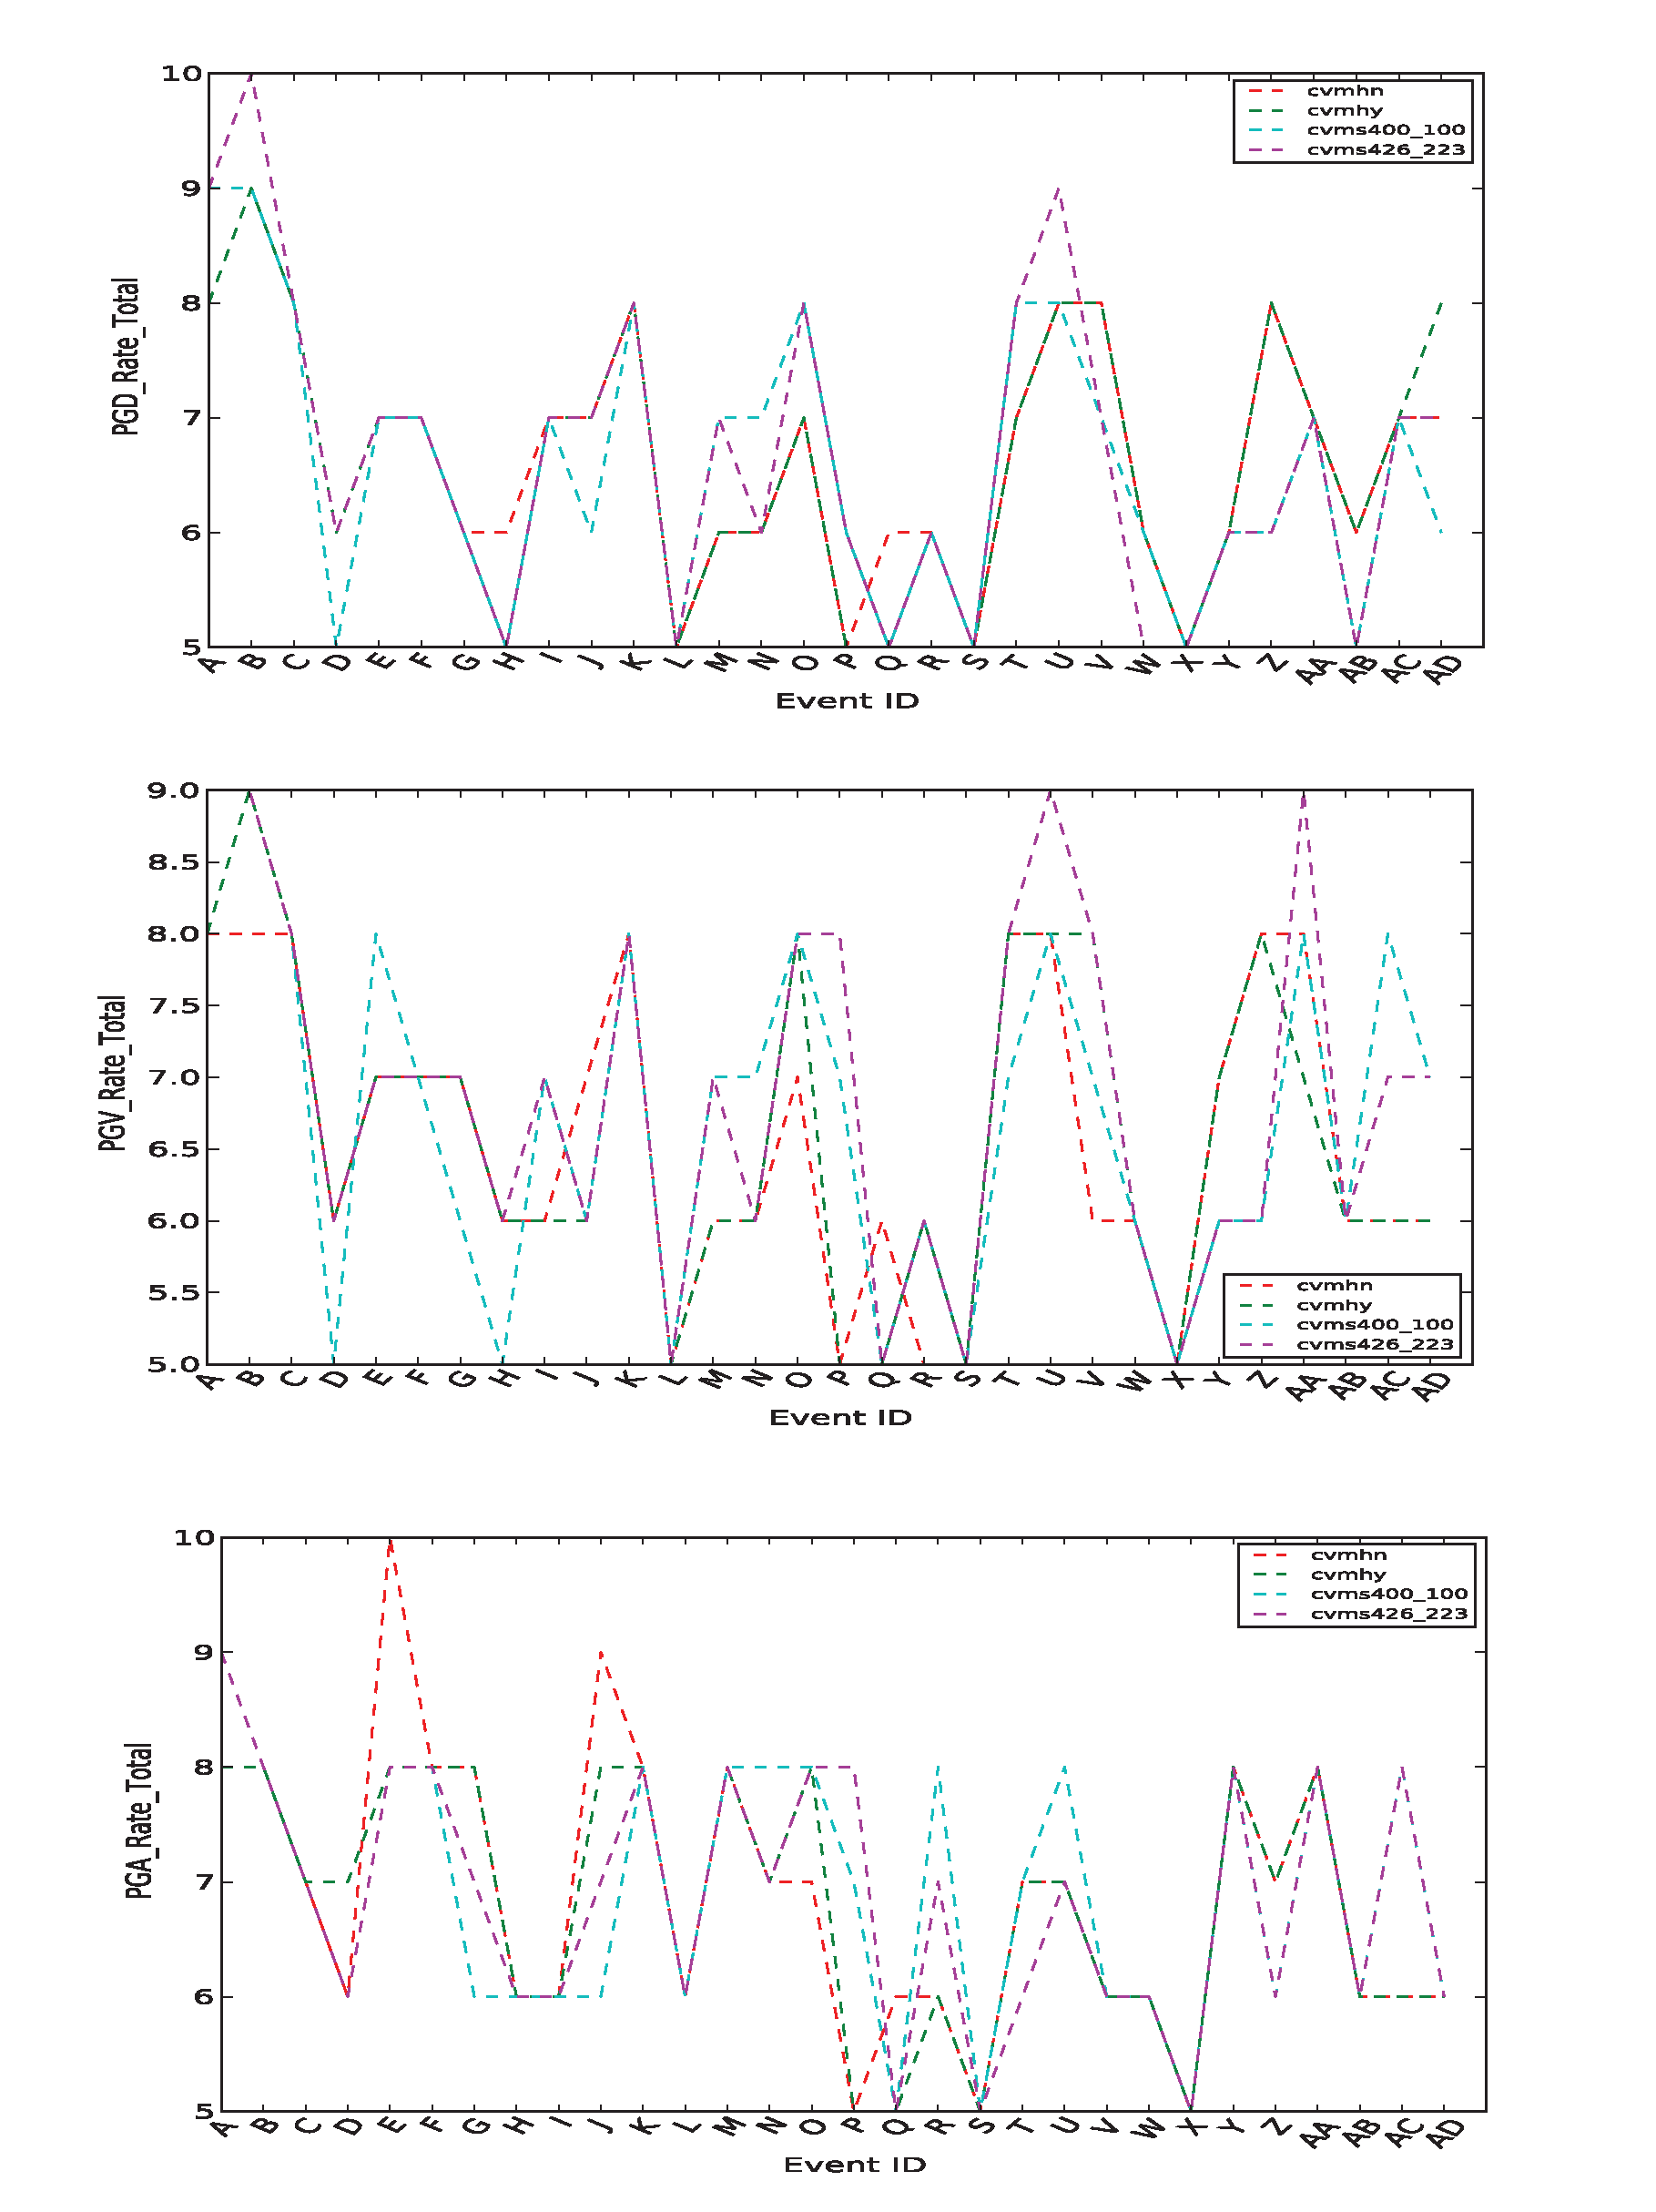
\includegraphics
    	[width=\textwidth]
    	{figures/pdf/figure-04}
    \caption{PGD, PGV and PGA rate score for all the 30 events and all four models are presented.}
    \label{fig:rate}
\end{figure*}

 Fig.~\ref{fig:score} shows trend of total average score for PGD, PGV and PGA for all 4 models. Again, the trend is similar, the score is better in PGD, then PGV, then PGA, and CVMS426-223 shows a better overall results.


\begin{figure*}
    \centering
    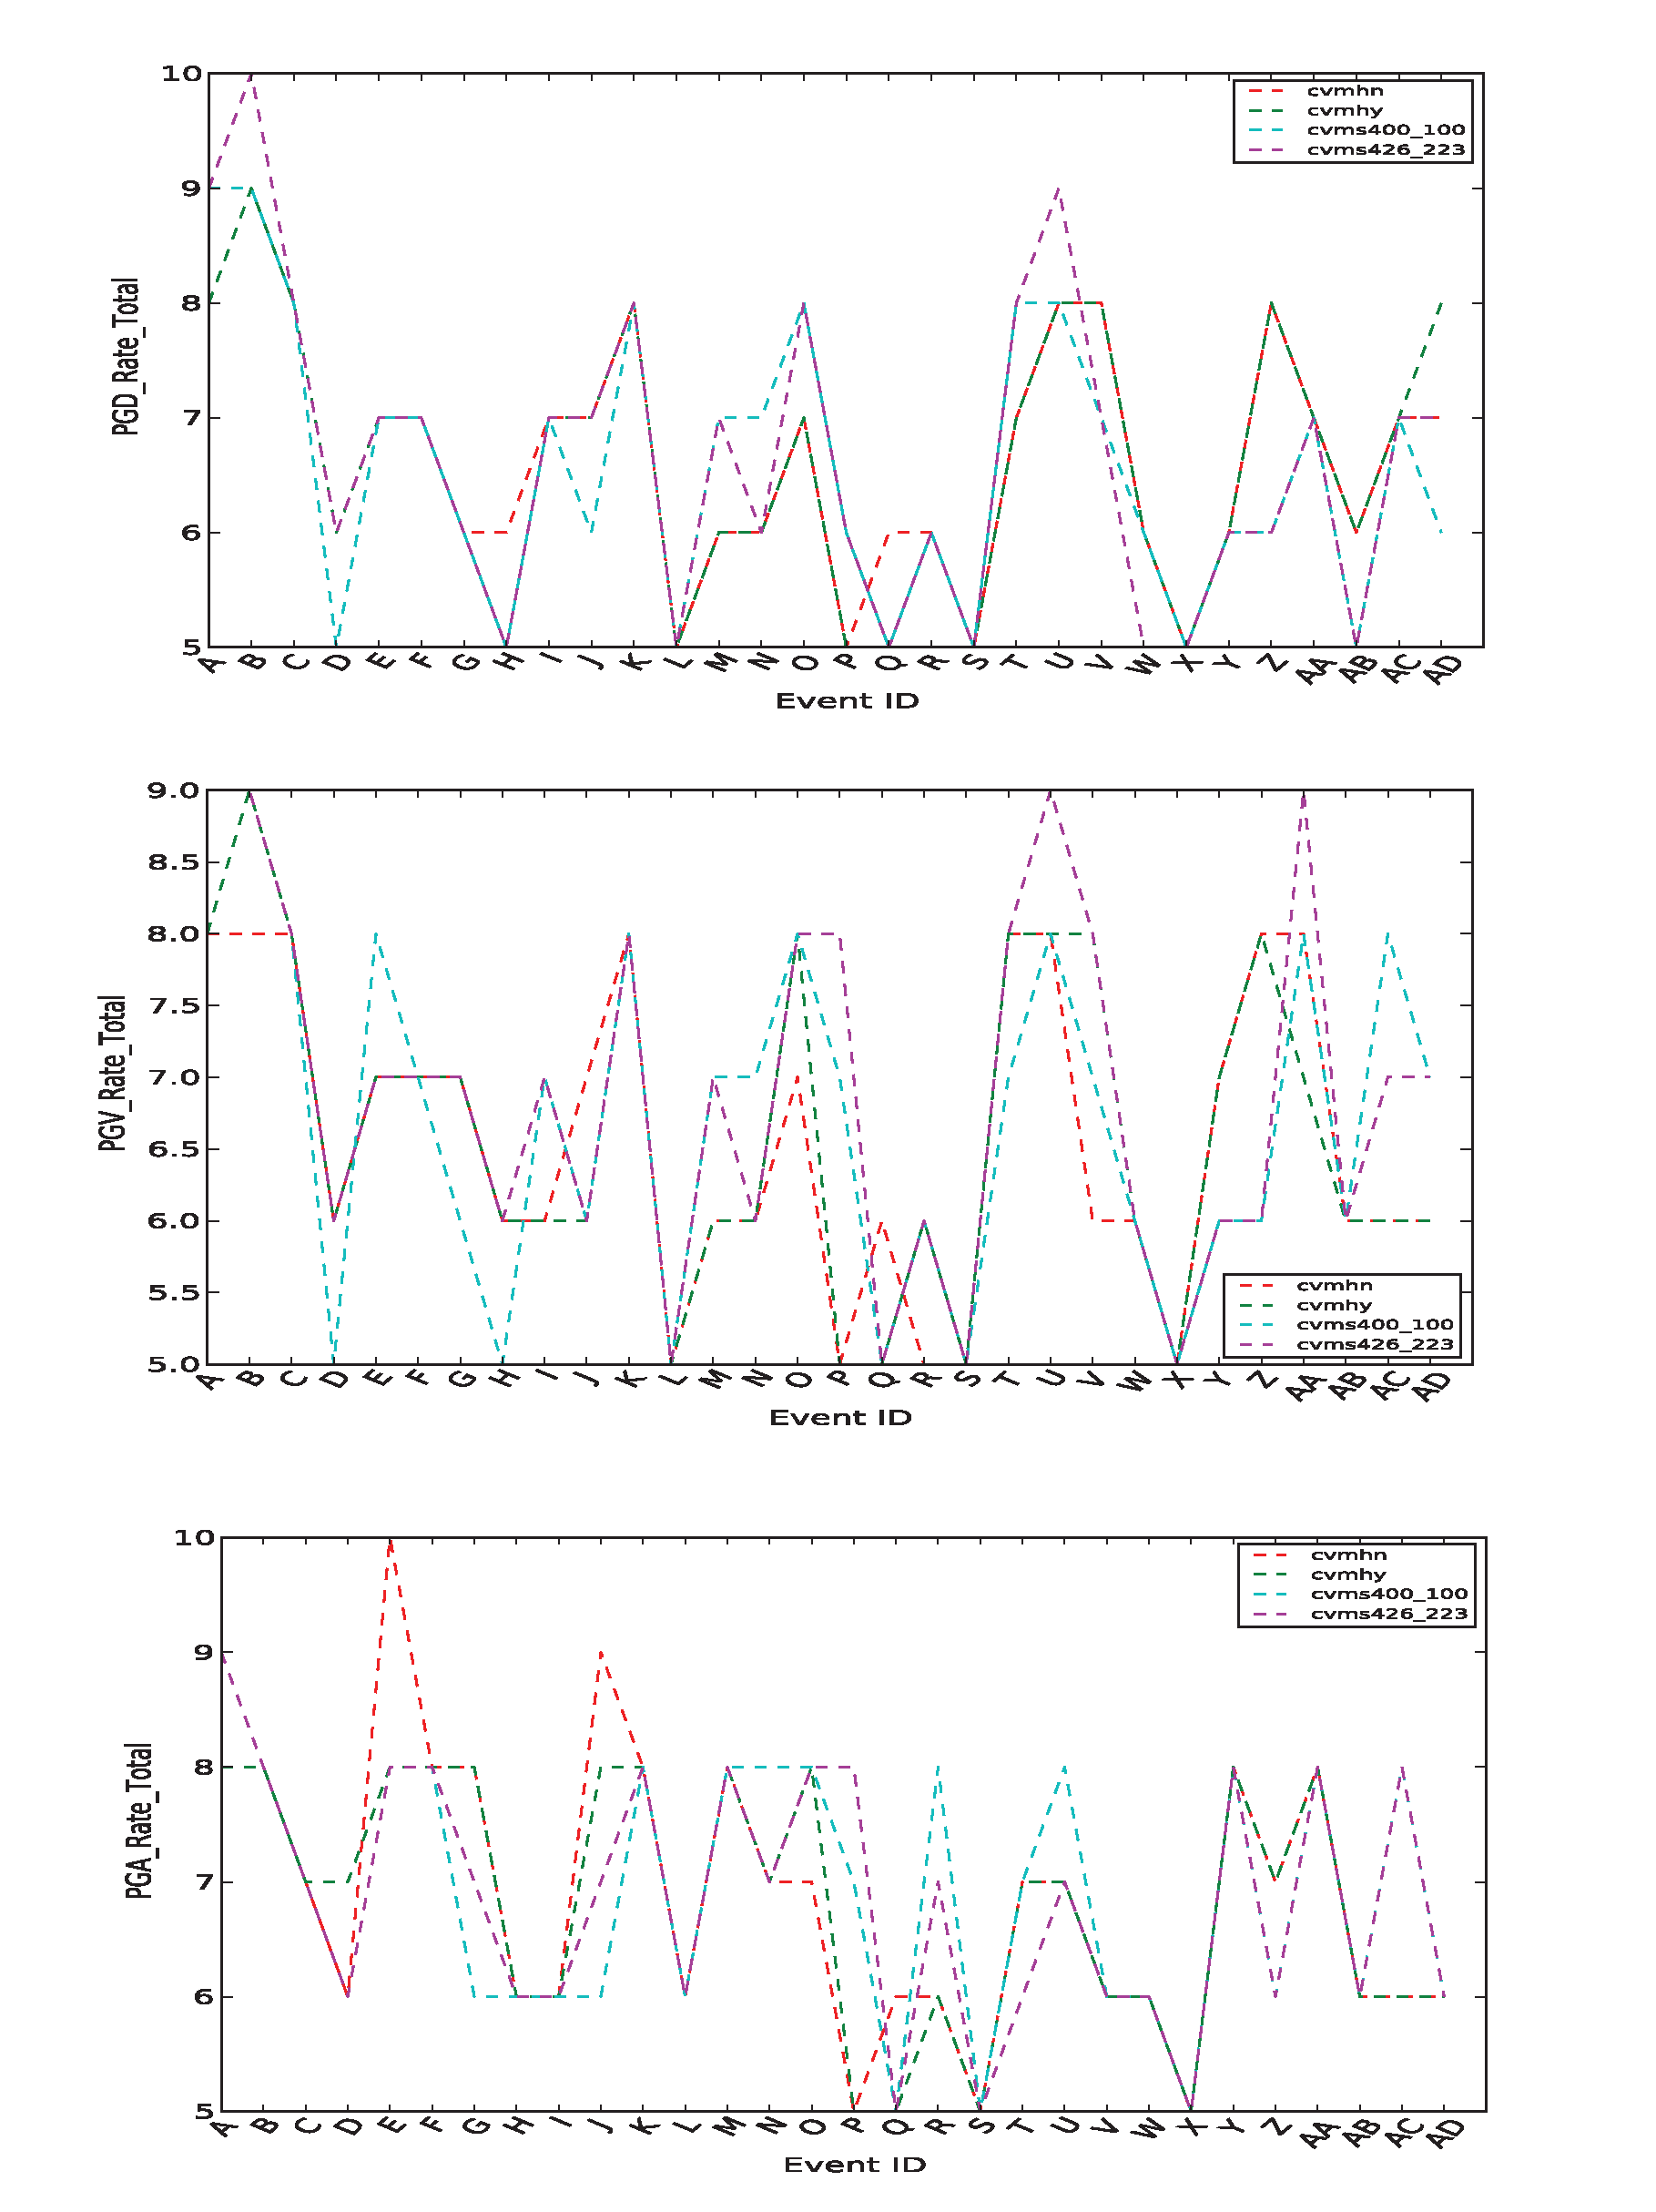
\includegraphics
    	[width=\textwidth]
    	{figures/pdf/figure-05}
    \caption{PGD, PGV and PGA total average score for all the 30 events and all four models are presented.}
    \label{fig:score}
\end{figure*}


A comparision between the latest results from scores of validation with modified anderson method and the method proposed here shows a good compatibility between final results of both methods. (See figure \ref{fig:comparision})

\begin{figure*}
    \centering
    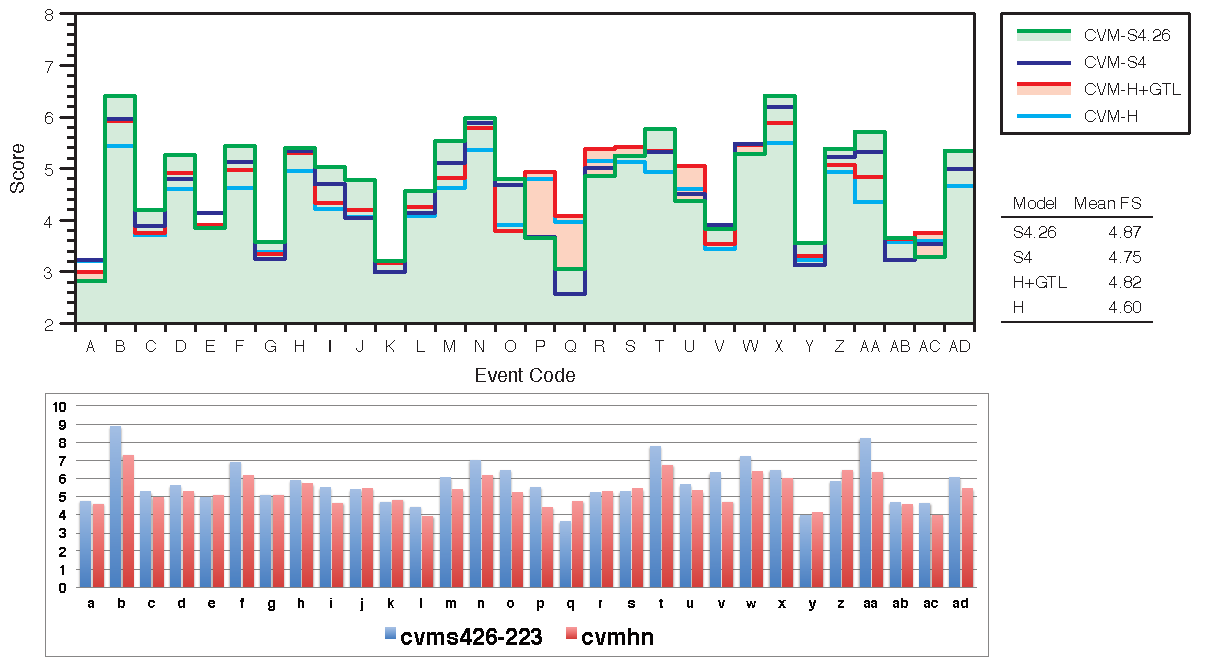
\includegraphics
    	[width=\textwidth]
    	{figures/pdf/figure-06}
    \caption{Results from modified Anderson score at top and the proposed score here for PGV at bottom}
    \label{fig:comparision}
\end{figure*}



\section{Further Works}

To improve the framework, here are some suggestions for the next steps. As it mentioned before, we can try to define the score directly according to the t value. So some different function will be tested to find an acceptable funcion.
Combination of amplitude and rate score can be done by simple average or by assigning weigh to each of the scores corrisponding to its importance. So that is something to work on.
Huge amount of data is available from the simulation domain area and we want to do the validation using all of those data. Similar procedure can be use with some modifications.The  comparisopns will be the same, except that it might be neceessary to select two different approximated lines for two different segments of the data and synthetics to get a more realistic approximation and more accurate results. In that case, the scores will be calculated for each segment separetely and then they will be combined with a simple or weighted average. In addition, with having many synthetic points, the amplitude score, instead of for each station, can be calculated in selected steps for the approximated line. The next step would be to check the results of synthetics with NGA predictions.






\bibliographystyle{gji}
\bibliography{references}
% \bsp 

\label{lastpage}

\end{document}
